% Paquets généraux
\documentclass[a4paper,12pt,titlepage]{article}
\usepackage[T1]{fontenc}
\usepackage[utf8]{inputenc}
\usepackage[french]{babel}
\usepackage[gen]{eurosym}
%\usepackage[dvips]{graphicx}
\usepackage{fancyhdr}
\usepackage{pdfpages} 
\usepackage{multido}
\usepackage{hyperref}
%\usepackage{textcomp}
%\usepackage{aeguill}
\usepackage{schemabloc}
\usepackage[bitstream-charter]{mathdesign}
\usepackage{minted}

\newcommand{\id}{71}
\newcommand{\nom}{Théorie des mécanismes}
\newcommand{\sequence}{04}
\newcommand{\nomsequence}{Liaisons entre les solides}
\newcommand{\num}{02}
\newcommand{\type}{KH}
\newcommand{\descrip}{Liaisons équivalentes, hyperstatisme, liaisons en série et en parallèle, théorie des graphes}
\newcommand{\competences}{B2-12: Proposer une modélisation des liaisons avec leurs caractéristiques géométriques. \\ &  B2-13: Proposer un modèle cinématique paramétré à partir d'un système réel, d'une maquette numérique ou d'u \\ &  B2-17: Simplifier un modèle de mécanisme. \\ &  B2-18: Modifier un modèle pour le rendre isostatique. \\ &  C1-04: Proposer une démarche permettant d'obtenir une loi entrée-sortie géométrique.  \\ &  C2-05: Caractériser le mouvement d'un repère par rapport à un autre repère. \\ &  C2-06: Déterminer les relations entre les grandeurs géométriques ou cinématiques. }
\newcommand{\nbcomp}{7}
\newcommand{\systemes}{}
\newcommand{\systemesnum}{}
\newcommand{\systemessansaccent}{}
\newcommand{\ilot}{2}
\newcommand{\ilotstr}{02}
\newcommand{\dossierilot}{\detokenize{Ilot_02 }}


\newcommand{\auteurun}{Renaud Costadoat}
\newcommand{\auteurdeux}{Françoise Puig}
\newcommand{\institute}{Lycée Dorian}


\usepackage{color}
\usepackage{xcolor}
\usepackage{colortbl}
\usepackage{helvet}
\usepackage[frenchmath]{newtxsf} % for sans serif symbols
\renewcommand{\familydefault}{\sfdefault}
%\usepackage{amsfonts}
%\usepackage{amsmath}
%\usepackage{lmodern}
\usepackage{mathastext}
%\usepackage{xspace}
\usepackage{varioref}
\usepackage{tabularx}
%\usepackage{floatflt}
\usepackage{graphics}
\usepackage{wrapfig}
\usepackage{textcomp}
\usepackage{tikz}
\usepackage{wrapfig}
\usepackage{gensymb}
\usepackage[european]{circuitikz}
\usetikzlibrary{babel}
\usepackage{ifthen}
\usepackage{cancel}
\usepackage{etoolbox}
\usepackage{multirow}
%\usepackage{boxedminipage}
\definecolor{gris25}{gray}{0.75}
\definecolor{bleu}{RGB}{18,33,98}
\definecolor{bleuf}{RGB}{42,94,171}
\definecolor{bleuc}{RGB}{231,239,247}
\definecolor{rougef}{RGB}{185,18,27}
\definecolor{rougec}{RGB}{255,188,204}%255,230,231
\definecolor{vertf}{RGB}{103,126,82}
\definecolor{vertc}{RGB}{220,255,191}
\definecolor{forestgreen}{rgb}{0.13,0.54,0.13}
\definecolor{blcr}{rgb}{0.59,0.69,0.84}
\definecolor{blfr}{rgb}{0.32,0.51,0.75}
\definecolor{orfr}{rgb}{0.90,0.42,0.15}
\definecolor{orcr}{rgb}{0.90,0.65,0.50}
\definecolor{orangef}{rgb}{0.659,0.269,0.072}
\definecolor{orange}{rgb}{0.58,0.35,0.063}
\definecolor{orangec}{rgb}{0.43,0.32,0.25}
\definecolor{rcorrect}{rgb}{0.6,0,0}
\definecolor{sequence}{rgb}{0.75,0.75,0.75}
\definecolor{competences}{rgb}{0.61,0.73,0.35}
\definecolor{grisf}{HTML}{222222}
\definecolor{grisc}{HTML}{636363}
\definecolor{normal}{HTML}{4087c4}
\definecolor{info}{HTML}{5bc0de}
\definecolor{success}{RGB}{92,184,92}
\definecolor{warning}{RGB}{240,173,78}
\definecolor{danger}{RGB}{217,83,79}
\hypersetup{                    % parametrage des hyperliens
    colorlinks=true,                % colorise les liens
    breaklinks=true,                % permet les retours à la ligne pour les liens trop longs
    urlcolor= blfr,                 % couleur des hyperliens
    linkcolor= orange,                % couleur des liens internes aux documents (index, figures, tableaux, equations,...)
    citecolor= forestgreen                % couleur des liens vers les references bibliographiques
    }

% Mise en page
\pagestyle{fancy}

\setlength{\hoffset}{-18pt}

\setlength{\oddsidemargin}{0pt} 	% Marge gauche sur pages impaires
\setlength{\evensidemargin}{0pt} 	% Marge gauche sur pages paires
\setlength{\marginparwidth}{00pt} 	% Largeur de note dans la marge
\setlength{\headwidth}{481pt} 	 	% Largeur de la zone de tête (17cm)
\setlength{\textwidth}{481pt} 	 	% Largeur de la zone de texte (17cm)
\setlength{\voffset}{-18pt} 		% Bon pour DOS
\setlength{\marginparsep}{7pt}	 	% Séparation de la marge
\setlength{\topmargin}{-30pt} 		% Pas de marge en haut
\setlength{\headheight}{35pt} 		% Haut de page
\setlength{\headsep}{20pt} 		% Entre le haut de page et le texte
\setlength{\footskip}{30pt} 		% Bas de page + séparation
\setlength{\textheight}{700pt} 		% Hauteur de l'icone zone de texte (25cm)
\setlength\fboxrule{1 pt}
\renewcommand{\baselinestretch}{1}
\setcounter{tocdepth}{1}
\newcommand{\cadre}[2]
{\fbox{
  \begin{minipage}{#1\linewidth}
   \begin{center}
    #2\\
   \end{center}
  \end{minipage}
 }
}

\newcounter{num_quest} \setcounter{num_quest}{0}
\newcounter{num_rep} \setcounter{num_rep}{0}
\newcounter{num_cor} \setcounter{num_cor}{0}

\newcommand{\question}[1]{\refstepcounter{num_quest}\par
~\ \\ \parbox[t][][t]{0.15\linewidth}{\textbf{Question \arabic{num_quest}}}\parbox[t][][t]{0.93\linewidth}{#1}\par
}


\newcommand{\reponse}[1]
{\refstepcounter{num_rep}
\noindent
\rule{\linewidth}{.5pt}
\textbf{Question \arabic{num_rep}:}
\multido{\i=1+1}{#1}{~\ \\}
}

\newcommand{\cor}
{\refstepcounter{num_cor}
\noindent
\rule{\linewidth}{.5pt}
\textbf{Question \arabic{num_cor}:} \\
}

\newcommand{\titre}[1]
{\begin{center}
\cadre{0.8}{\huge #1} 
\end{center}
}


% En tête et pied de page
\fancypagestyle{normal}{%
  \fancyhf{}
\lhead{\nom}
\rhead{
\includegraphics[width=2cm]{../../img/logo}\hspace{2pt}}
\ifdef{\auteurdeux}{\lfoot{\auteurun,\auteurdeux}}{\lfoot{\auteurun}}
\cfoot{Page \thepage}}

\fancypagestyle{correction}{%
  \fancyhf{}
  \lhead{\colorbox{danger}{\begin{minipage}{0.65\paperwidth} \textcolor{white}{\textbf{Correction}} \end{minipage}} }
  \rhead{
\includegraphics[width=2cm]{../../img/logo}}
  \ifdef{\auteurdeux}{\lfoot{\auteurun,\auteurdeux}}{\lfoot{\auteurun}}
  \rfoot{\colorbox{danger}{\begin{minipage}{0.5\paperwidth} \begin{flushright}\textcolor{white}{\textbf{Correction}}\end{flushright} \end{minipage}} }}

\renewcommand{\footrulewidth}{0.4pt}

\usepackage{eso-pic}
\newcommand{\BackgroundPic}{%
\put(0,0){%
\parbox[b][\paperheight]{\paperwidth}{%
\vfill
\begin{center}
\hspace{0.5cm}\vspace{0.5cm}

\includegraphics[width=\paperwidth,height=\paperheight,%
keepaspectratio]{../../img/fond3}%
\end{center}
\vfill
}}}

\newcommand{\BackgroundPicdeux}{%
\put(25,-30){%
\parbox[b][\paperheight]{\paperwidth}{%
\vfill
\begin{center}

\includegraphics[width=\paperwidth,height=\paperheight,%
keepaspectratio]{../../img/fond4}%
\end{center}
\vfill
}}}

\begin{document}

\pagestyle{empty}

\vspace*{-3\baselineskip}

\AddToShipoutPicture*{\BackgroundPic}

\ifdef{\auteurdeux}{\begin{tabular}{>{\columncolor{gray!00}}m{.3\linewidth} m{.3\linewidth} >{\columncolor{gray!00}}m{.3\linewidth}}
Séquence : \sequence &  \multirow{3}{*}{\hspace{1cm}
\includegraphics[height=1.5cm]{../../img/logo}} &  \begin{flushright} \multirow{4}{*}{\hspace{1cm}\includegraphics[height=4cm]{img/qrcode}}\end{flushright}\\
Document : \type\num \\
 \institute \\
 \auteurun\\
 \auteurdeux
\end{tabular}}{\begin{tabular}{>{\columncolor{gray!00}}m{.3\linewidth} m{.3\linewidth} >{\columncolor{gray!00}}m{.3\linewidth}}
Séquence : \sequence &  \multirow{3}{*}{\hspace{1cm}
\includegraphics[height=1.5cm]{../../img/logo}} &  \begin{flushright} \multirow{4}{*}{\hspace{1cm}\includegraphics[height=4cm]{img/qrcode}}\end{flushright}\\
Document : \type\num \\
 \institute \\
 \auteurun
\end{tabular}}

\vspace{1cm}

\ifdef{\prive}{\begin{center}\colorbox{danger}{\Huge{Avec Correction}}\end{center}}{}

\begin{center}\huge{\nom}\end{center}

\vspace{2cm}

\ifdef{\imagedeux}{\begin{minipage}{0.49\linewidth}}{}
\begin{center}\includegraphics[height=5cm]{/home/renaud/Documents/Renaud/GitHub/django_education/systemes/\imageun}\end{center}
\ifdef{\imagedeux}{\end{minipage}\hfill
\begin{minipage}{0.49\linewidth}
\begin{center}\includegraphics[height=5cm]{/home/renaud/Documents/Renaud/GitHub/django_education/systemes/\imagedeux}\end{center}
\end{minipage}}{}

\vspace{5cm}


\begin{tabular}{p{.15\linewidth} >{\columncolor{white}}p{.8\linewidth}}
    \rowcolor{gray!20}
    Référence & S\sequence\ - \type\num \\
    Compétences & \competences \\
 	\rowcolor{gray!20}
    Description & \descrip \\
    Système & \systemes
  \end{tabular}

\newpage

\AddToShipoutPicture{\BackgroundPicdeux}

\pagestyle{normal}


\section{Palettiseur de gobelets}


Mise en situation
L'entreprise VMC (Verrerie Mécanique Champenoise), filiale du groupe BSN, transforme, grâce à ses deux fours, 600 tonnes de verre par jour en différents articles tels que : bocaux, flacons et gobelets (verres à eau, verres à moutarde, verres mesureurs,...). Le nombre d'articles fabriqués est de 2 à 5 millions par jour (24 heures par jour et 365 jours par an). On n'arrête jamais un four de fusion de verre.

Les articles sont moulés automatiquement dans des moules métalliques, puis ils subissent un recuit permettant de diminuer leur fragilité. Ces articles sont ensuite contrôlés à 100\% (aspect, dimensions et géométrie) puis convoyés vers les palettiseurs.

Chaque ligne de fabrication possède son propre palettiseur. La fonction globale de ce palettiseur est de ranger un maximum d'articles en différentes couches sur une palette normalisée (1m x 1,2m). Le type de rangement et le nombre de couches est défini par un cahier des charges.

Pour terminer, les palettes passent dans une housseuse afin d'être recouvertes d'une housse en matière plastique absolument étanche à la pluie et aux différentes poussières. Les palettes houssées sont ensuite expédiées chez le client.

Les gobelets triés et contrôlés arrivent par le convoyeur d'amenée. Ce convoyeur, actionné par un moteur électrique, avance continuellement. Lorsque le nombre de gobelets formant une ligne est atteint, un bloqueur pneumatique (V1) arrête l'arrivée des articles. Le TAA (Transporteur Automatique d'Articles), actionné par un vérin pneumatique (V2), transfère la ligne de gobelets sur la table d'accumulation et pousse les lignes déjà en place. Ainsi de suite jusqu'à la formation
d'une couche complète.

\begin{minipage}{0.48\linewidth}
Les gobelets sont ici rangés suivant le modèle ci contre.
\begin{itemize}
 \item Nombre pair de gobelets sur la première ligne (Np).
 \item Nombre impair de gobelets sur la deuxième ligne (Ni)
 \item \og Quinconçage \fg des articles (vérin V3).
 \item Il y a un nombre impair de lignes.
\end{itemize}
\end{minipage}
 \hfill
\begin{minipage}{0.38\linewidth}
 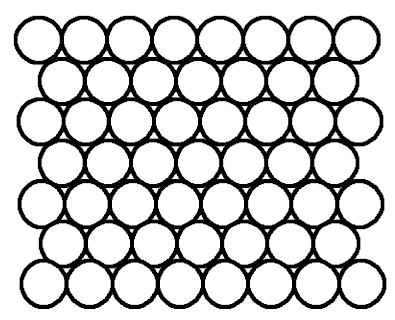
\includegraphics[width=0.5\linewidth]{img/Rangement.png}
\end{minipage}

Lorsqu'une couche est formée, le plateau du TAC (Transporteur Automatique de Couches), actionné par des vérins pneumatiques, prend la couche (création d'un vide entre le plateau et les gobelets) et la transfère sur la palette en cours de formation. Il revient ensuite à sa position d'attente sous la table d'accumulation.

Lorsqu'une couche est déposée par le TAC et qu'il est reparti, le TAI (Transporteur Automatique d'Intercalaires), actionné par des vérins pneumatiques (non représentés sur le document 1), vient placer un intercalaire en carton ondulé sur la couche afin de l'isoler de la suivante.

Lorsque l'intercalaire est mis en place sur la couche, le plateau de la table élévatrice descend de la hauteur d'une couche. Cette table est équipée d'un groupe hydraulique autonome actionné par un moteur électrique.

Lorsque le nombre de couches est atteint, la palette pleine est évacuée par le convoyeur de palettes vers la housseuse. Une autre palette vide garnie d'un film plastique peut se présenter sur le plateau de la table élévatrice. Les convoyeurs de palettes sont actionnés par des moteurs électriques.


\subsection{Étude automatique}

Objectifs :
\begin{itemize}
 \item Commencer l'étude d'un système combinatoire permettant de comparer deux codes binaires.
 \item Étudier le diagramme d'activité de formation d'une couche de gobelets avant palettisation.
\end{itemize}

\subsection{Combinatoire}

Depuis que l'entreprise est certifiée ISO 9001, le responsable de la chaine de conditionnement doit composer un code personnel a 4 chiffres afin d'assurer la traçabilité du conditionnement. Ce code, figure, entre autres, sous forme de code barres sur une étiquette collée sur la palette.

Le code est entre dans l'étiqueteuse par l'intermédiaire d'un clavier. Les codes des différents responsables sont mémorisés dans la machine. Le code entre au clavier est compare aux codes mémorisés afin de vérifier sa conformité.

\paragraph{Question 1:} Le code entre au clavier est tel que : $0000 \leq code \leq 9999$. On décide dans un premier temps de transformer ce nombre a quatre chiffres en un mot binaire naturel, combien le mot binaire doit-il comporter de bits ?

\paragraph{Question 2:} Tracer le logigramme de $a \oplus b$ avec des opérateurs NAND (NON-ET) a deux entrées.

\paragraph{Question 3:} Montrer que $\overline{a \oplus b} = \overline{a}.\overline{b} + a.b$. Établir la table de vérité. Donner le nom de cet opérateur.

Ce type de codage en binaire naturel étant peu pratique, on retient le codage \og DCB \fg, nécessitant 16 bits, dans lequel chaque chiffre du code est représente par son équivalent en binaire naturel (exemple : $9245_{10} = 1001 0010 0100 0101_{DCB})$.

On ne s'intéresse dans la question suivante qu'au chiffre des unités. On note \textbf{xyzt}, l'équivalent binaire du chiffre des unités du code entre au clavier et \textbf{abcd} l'équivalent binaire du chiffre des unités de l'un des codes mémorisés dans l'étiqueteuse.

\paragraph{Question 4:} Déterminer \textbf{F(x,y,z,t,a,b,c,d)}, une fonction binaire caractérisant l'égalité entre les deux mots \textbf{xyzt} et \textbf{abcd}. $(\textbf{F} = 1, \textbf{xyzt} = \textbf{abcd} et \textbf{F} = 0, \textbf{xyzt} \neq \textbf{abcd})$

\subsection{Séquentiel}

Conditions initiales :
\begin{itemize}
 \item le convoyeur d'amenée fonctionne en continu ;
 \item le vérin \textbf{V1}, tige sortie, bloque les gobelets, il n'y a pas de gobelets en face du \textbf{TAA}. Il y a glissement entre les gobelets et le tapis du convoyeur d'amenée ;
 \item la tige du vérin \textbf{V2} est rentrée ;
 \item la tige du vérin \textbf{V3} est rentrée ;
 \item le \textbf{TAC} et le \textbf{TAI} sont dans la position du document 1.
\end{itemize}

Marche automatique :
\begin{itemize}
 \item le vérin \textbf{V1}, tige rentrée laisse passer les gobelets ;
 \item quand la cellule de comptage a compté \textbf{Ni} (nombre impair de gobelets) ou \textbf{Np} (nombre pair de gobelets), la tige de \textbf{V1} sort pour bloquer les gobelets ;
 \item la ligne de gobelets étant formée, le vérin \textbf{V2} pousse la ligne sur la table d'accumulation ;
 \item pendant le retour de \textbf{V2}, le vérin \textbf{V3} prend la position (tige sortie) d'une ligne impaire de
gobelets ;
 \item si la cellule de fin de couche cf de la table d'accumulation détecte qu'une couche de gobelets est formée, le \textbf{TAC} vient saisir la couche et la dépose sur la palette en cours de formation;
 \item quand cette opération est terminée, une nouvelle couche de gobelets peut être formée.
\end{itemize}
 
Données supplémentaires :
\begin{itemize}
 \item la première et la dernière ligne d'une couche sont toujours des lignes paires. Il y a un nombre impair de lignes dans une couche ;
 \item tous les vérins sont à double effet et à commande bistable électrique;
 \item on doit attendre 0,5 s après que \textbf{V1} soit en position sortie pour pousser la ligne formée ;
 \item on doit attendre le signal de fin d'évacuation de la couche avant de commencer la formation d'une nouvelle couche.
\end{itemize}

Les étapes ont été numérotées pour plus de lisibilité.

 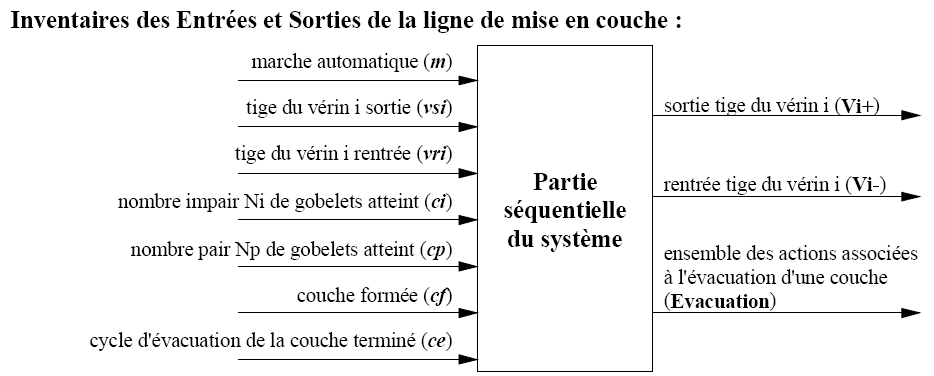
\includegraphics[width=0.7\linewidth]{img/Inventaire.png}

\paragraph{Question 5 :} Donner les réceptivités associées aux transitions \textbf{t2}, \textbf{t5}, \textbf{t5'}, \textbf{t7}, \textbf{t10} et \textbf{t11}.

On note \textbf{Pi+}, la position du distributeur relative à la sortie de la tige du piston du vérin \textbf{Vi} et \textbf{Pi-} la position du distributeur relative à la rentrée de la tige du piston du vérin \textbf{Vi}.

On rappelle que \textbf{V2-} et \textbf{V2+} représentent les variables booléennes associées aux commandes des bobines des distributeurs. Niveau logique 1 quand la bobine est excitée, 0 quand elle ne l'est pas.

\paragraph{Question 6 :} On se place dans le contexte de l'étape 5. Compléter le schéma suivant relatif au vérin V2 et à son distributeur : représenter le piston du vérin et le raccordement au distributeur.

~\

\begin{center}
 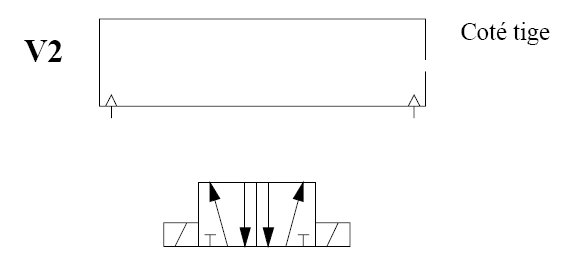
\includegraphics[width=0.5\linewidth]{img/R1.png}
\end{center}

Préciser à l'aide d'une flèche le sens de déplacement du piston. Indiquer si le distributeur est en position \textbf{P2+} ou \textbf{P2-}. Donner la désignation de ce distributeur.

\paragraph{Question 7 :} Compléter le chronogramme suivant par les niveaux logiques de \textbf{V2-} et \textbf{V2+} et par les positions du distributeur du vérin \textbf{V2}.

\begin{center}
 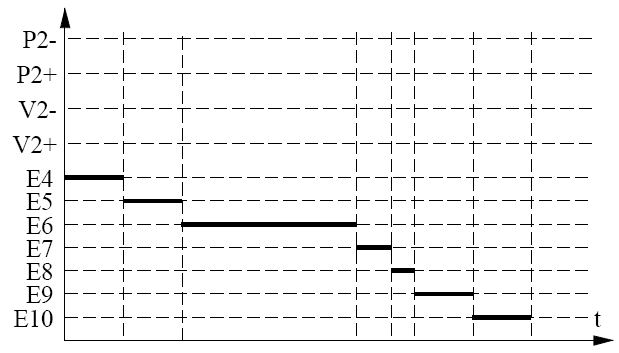
\includegraphics[width=0.6\linewidth]{img/R2.png}
\end{center}

\begin{center}
 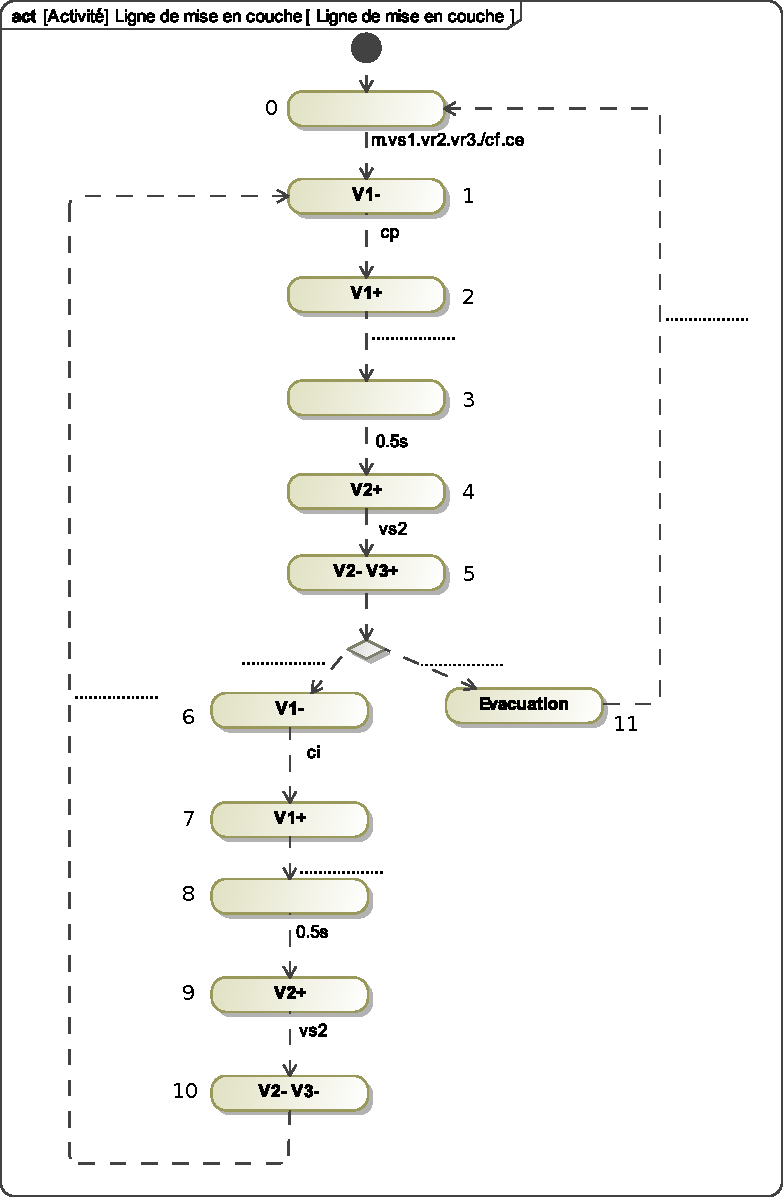
\includegraphics[width=0.6\linewidth]{img/Ligne_couche}
\end{center}

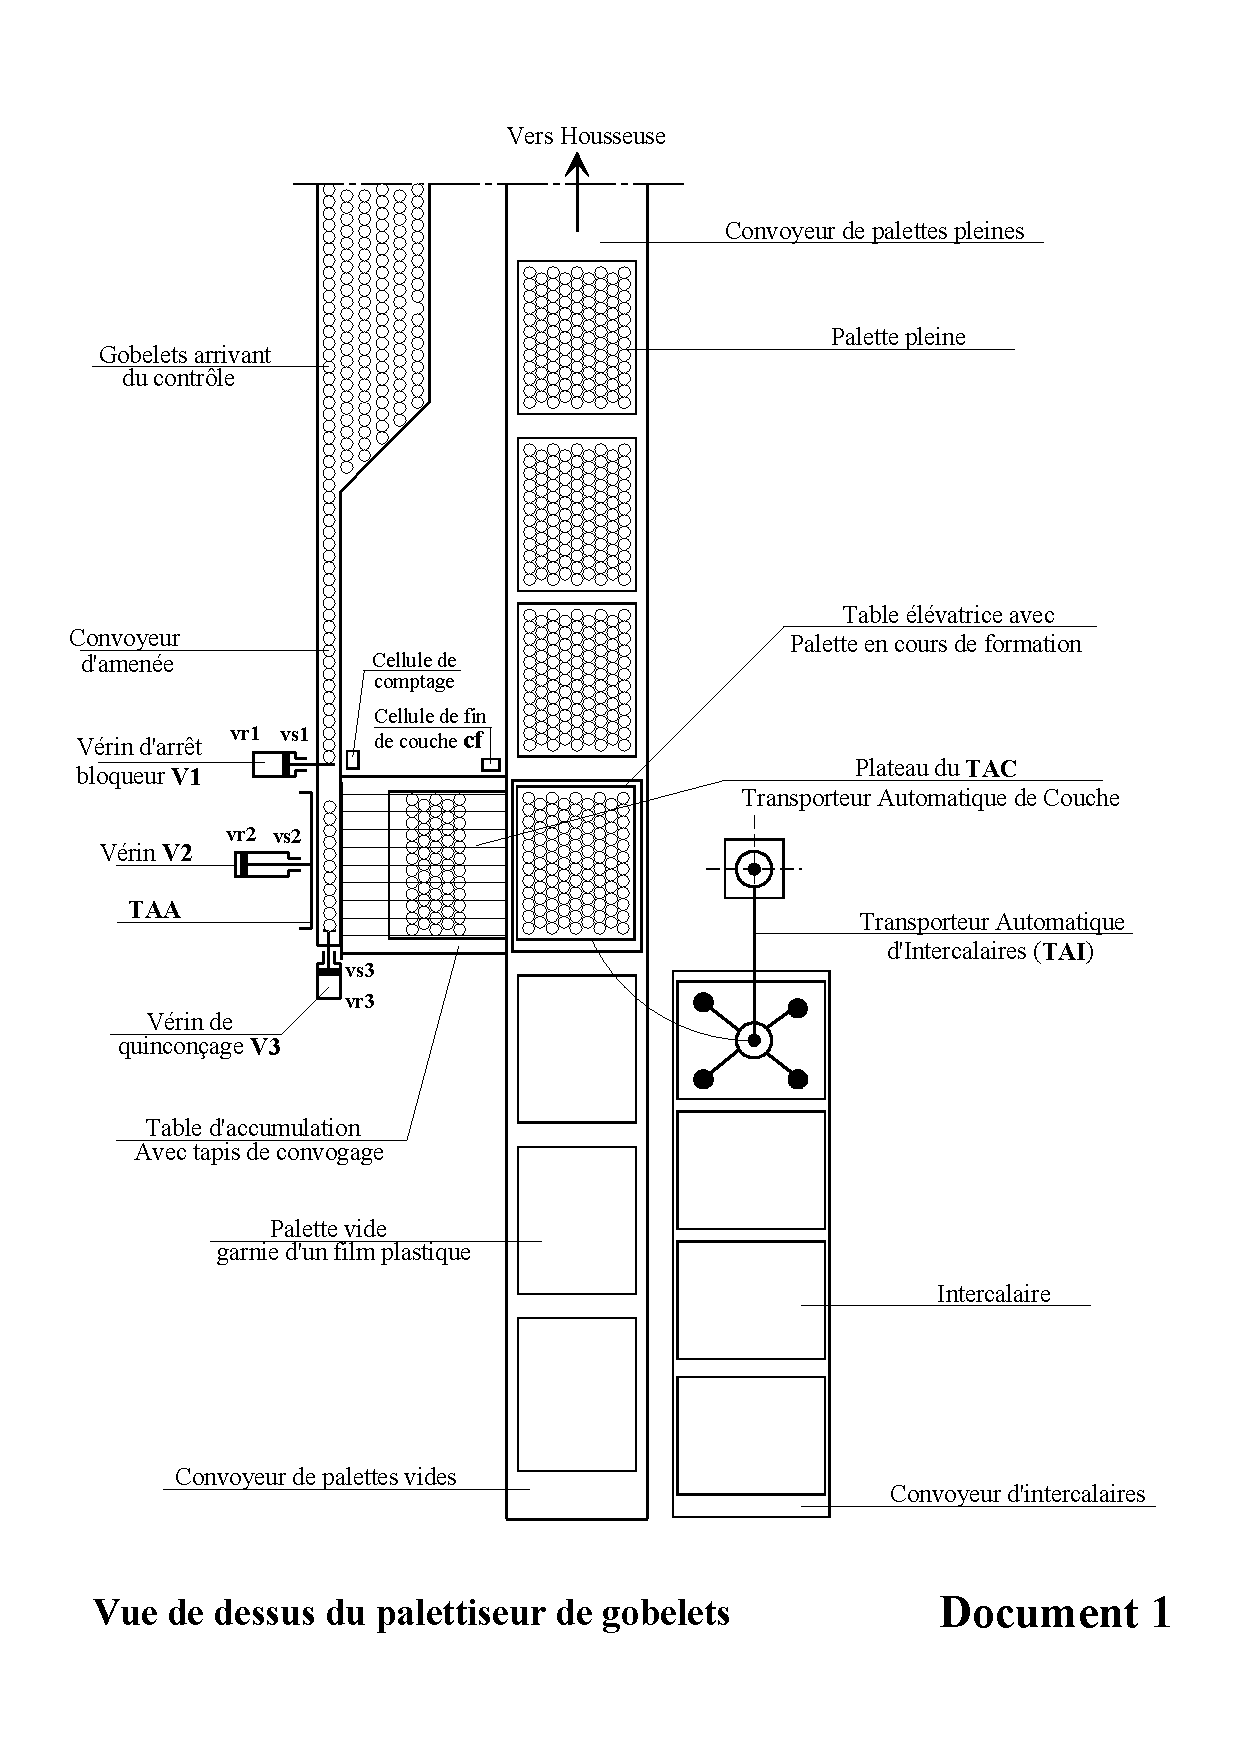
\includepdf{img/S1-D1-05.pdf}

\section{Robot robuglass}

\subsection{Analyse du système étudié}

La société ROBOSOFT a développé un robot devant assurer de manière automatique l'entretien de la pyramide du Louvre sans nécessiter l'intervention (difficile et périlleuse) des opérateurs directement sur l'édifice comme cela était le cas auparavant. Grand édifice de verre et d'acier (20 mètres de hauteur pour 35 mètres de côté), la pyramide du Louvre
est emblématique du musée à plus d'un titre puisqu'elle constitue également son entrée principale, son état doit donc être irréprochable. Le robot dénommé ROBUGLASS développé par la société ROBOSOFT s'inspire des machines utilisées pour le lavage des sols utilisant une brosse tournante et un dispositif de raclage. La forte déclivité des faces de la pyramide, les surfaces glissantes sur lesquelles le robot doit évoluer, et la volonté de le rendre automatique pour un
nettoyage rapide et optimal ont soulevé de nombreuses problématiques que nous allons en partie aborder.

Le robot ROBUGLASS se compose de 4 sous ensembles distincts (voir Annexe 1, Figure 1) :
\begin{itemize}
 \item le porteur : qui constitue le robot qui se déplace sur la surface vitrée, emportant l'outil de nettoyage. L'outil de nettoyage est constitué d'une brosse, d'une buse qui l'arrose de produit nettoyant et d'un dispositif de raclage (raclette + essuie glace).
 \item le chariot ombilical : qui supporte les 2 pompes à vide (assurant une redondance pour des raisons de sécurité) et auquel sont connectées toutes les sources d'énergie provenant du véhicule atelier.
 \item le poste de contrôle : qui permet à l'opérateur de commander manuellement le porteur ou de vérifier le bon déroulement de l'opération de nettoyage.
 \item le véhicule atelier : qui permet le rangement du porteur, de l'outillage et du chariot ombilical. Il contient une cuve avec sa pompe pour la préparation et le transfert du produit de nettoyage. Il permet de réaliser l'entretien courant et les petites réparations.
\end{itemize}

\subsection{Réalisation de la partie commande en mode automatique}

Initialement, le robot est positionné manuellement par l'opérateur en bas à gauche d'une face de la pyramide, de telle façon que le capteur de détection du joint gauche se situe à droite du joint (Annexe 6, Figure 10). Le centre de gravité du robot se situe au point A (Annexe 7, Figure 11). En mode automatique, le robot obéit au déroulement des opérations suivantes pour laver une travée (Annexe 7, Figure 11) :
\begin{itemize}
 \item Montée en changeant de trajectoire vers la droite pour rejoindre et s'aligner sur le joint gauche sans application de l'outil de nettoyage (point B).
 \item Montée sur une travée de vitres en suivant le joint de vitre gauche sans application de l'outil de nettoyage.
 \item Arrêt du robot à la détection de l'extrémité haute de la pyramide (point C).
 \item Descente du robot en suivant le joint de gauche en appliquant l'outil de nettoyage. La descente débute après l'application de l'outil.
 \item Arrêt du robot à la détection de l'extrémité basse de la pyramide (point D).
 \item Montée en changeant de trajectoire vers la droite pour rejoindre et s'aligner sur le joint droit sans application de l'outil de nettoyage (point E).
 \item Montée en suivant le joint droit sans application de l'outil de nettoyage.
 \item Arrêt du robot à la détection de l'extrémité haute de la pyramide (point F).
 \item Descente du robot en suivant le joint de droite en appliquant l'outil de nettoyage. La descente débute après l'application de l'outil.
 \item Arrêt du robot à la détection de l'extrémité basse de la pyramide (point G).
 \item Montée en changeant de trajectoire pour changer de travée de vitre et pour rejoindre le joint gauche de cette nouvelle travée sans application de l'outil de nettoyage (point H).
 \item Etc...
\end{itemize}

Pour permettre ce fonctionnement, le robot est équipé d'un certain nombre de capteur, dont :
\begin{itemize}
 \item capteur de détection de la partie basse de la travée associée à la variable binaire : \textbf{pb}
 \item capteur de détection de la partie haute de la travée associée à la variable binaire : \textbf{ph}
 \item capteur de détection et d'alignement sur le joint de gauche de la travée associée à la variable binaire : \textbf{pg}
 \item capteur de détection et d'alignement sur le joint de droite de la travée associée à la variable binaire : \textbf{pd}
 \item capteur de détection de la position haute de l'outil associée à la variable binaire : \textbf{oh}
 \item capteur d'information de la bonne application de l'outil sur la surface vitrée associée à la variable binaire : \textbf{ob}
\end{itemize}

Par ailleurs un certain nombre de variable permettent de commander le robot :
\begin{itemize}
 \item \textbf{M} commande monostable de l'asservissement en suivi de joint du robot sur la travée en phase de montée.
 \item \textbf{D} commande monostable de l'asservissement en suivi de joint du robot sur la travée en phase de descente.
 \item \textbf{R} commande monostable de l'asservissement du robot pour prendre un virage à droite et s'aligner sur le nouveau joint qu'il détecte (joint de gauche ou joint de droite).
 \item \textbf{L} commande monostable permettant d'actionner l'outil.
 \item \textbf{AL} envoie un signal d'alarme à l'opérateur en cas de défaillance détectée. Dans ce cas, le robot doit passer en mode manuel pour pouvoir se déplacer à nouveau.
\end{itemize}

Le diagramme d'état de coordination des taches est donné en Annexe 7, Page 12.

\newpage

\paragraph{Question 1:} Compléter le diagramme d'activités correspondant au lavage d'une seule travée. Ce diagramme d'activité indépendant est activé lorsque l'état "Lavage d'une travée" du diagramme d'état de coordination des taches est actif.

\vspace{2cm}

\begin{center}
 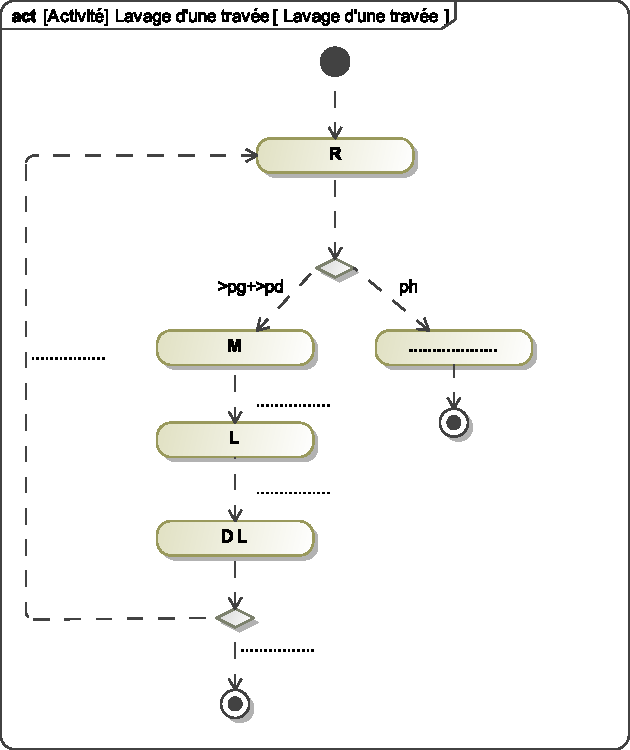
\includegraphics[width=0.7\linewidth]{img/Lavage_travee}
\end{center}

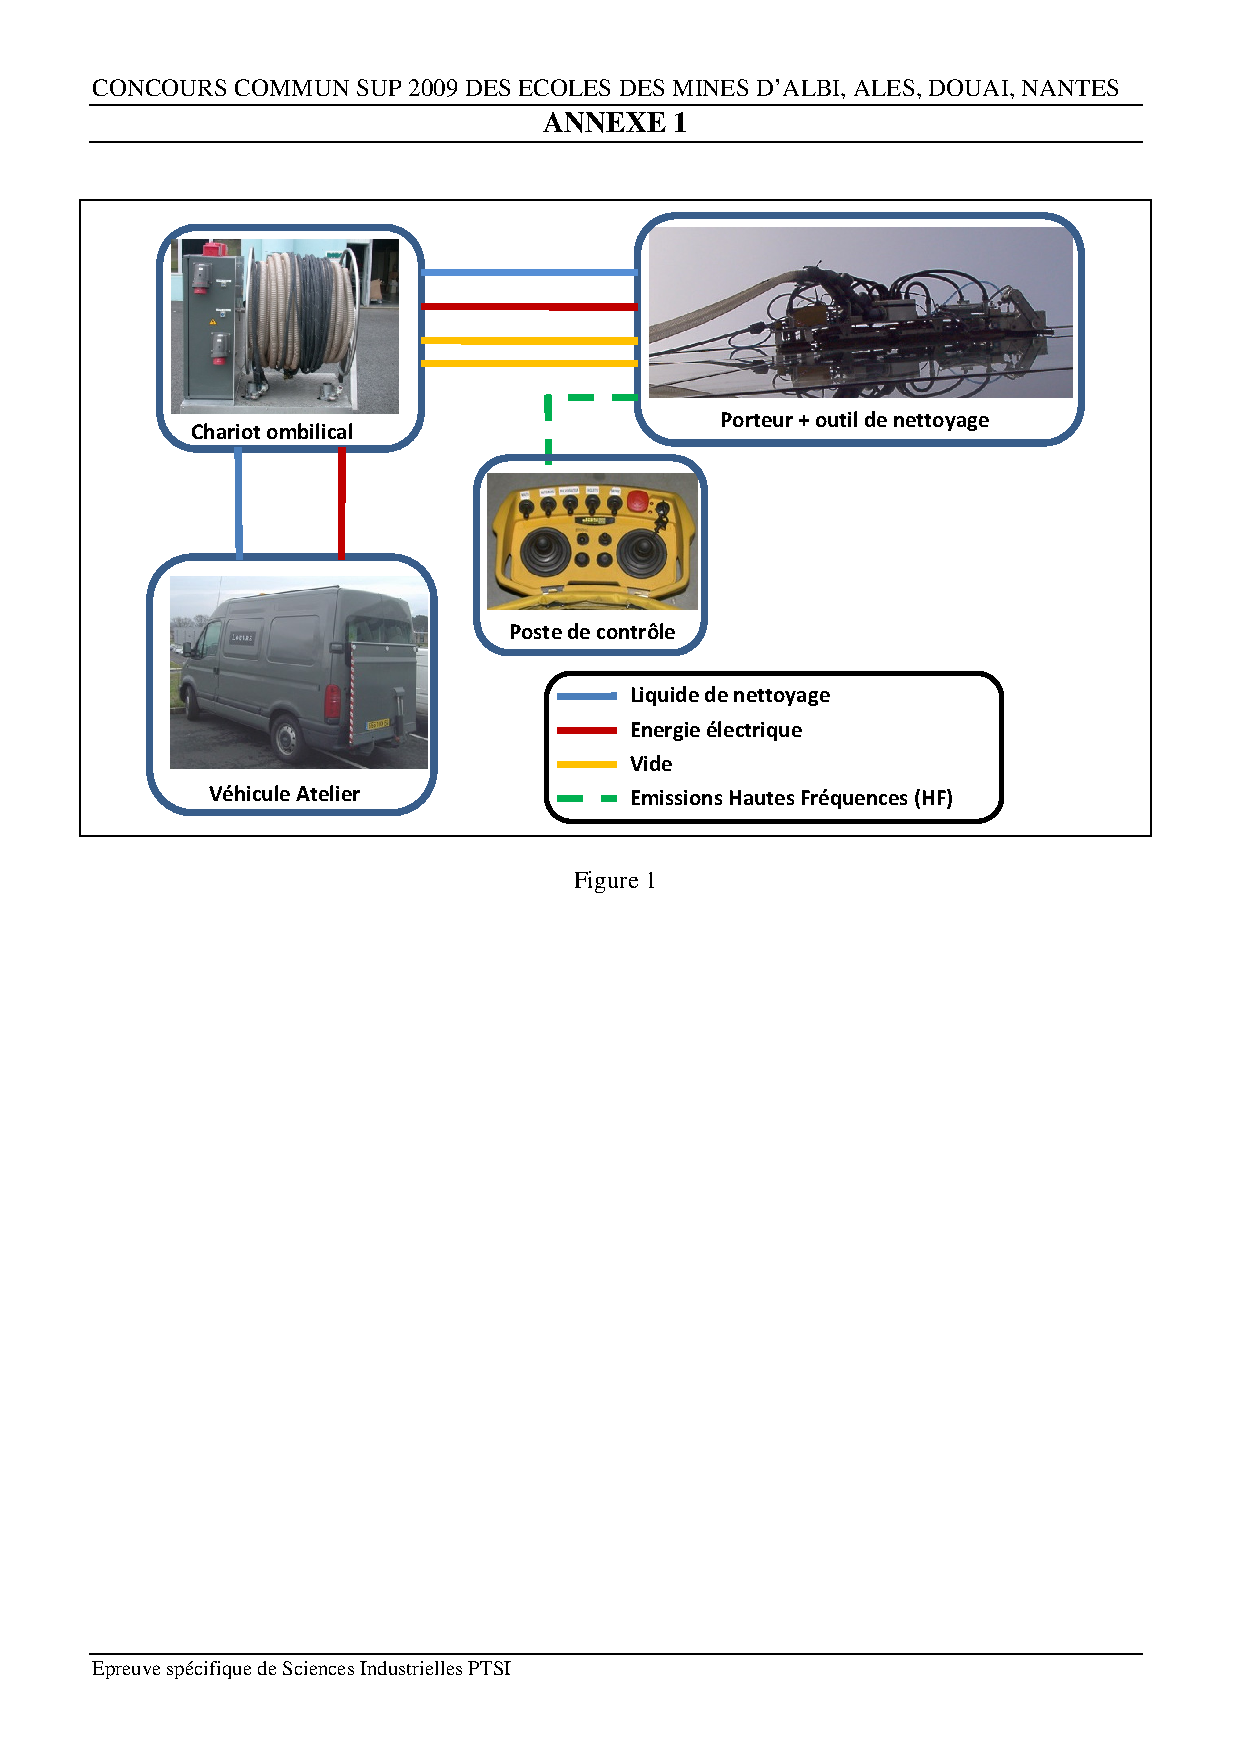
\includepdf[pages=1]{img/S2-D1-D8-09.pdf}

\includepdf[pages=6]{img/S2-D1-D8-09.pdf}

\begin{center}
 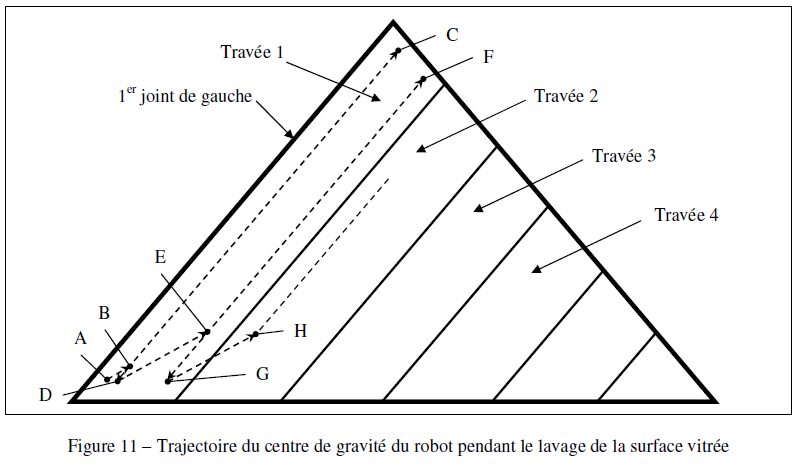
\includegraphics[width=0.7\linewidth]{img/Figure11}
  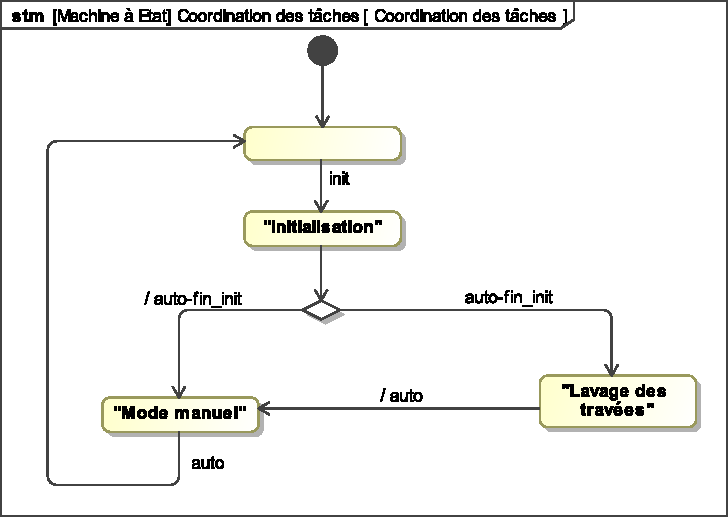
\includegraphics[width=0.7\linewidth]{img/Coordination_taches}
\end{center}

\newpage

\section{Traitement de surface}


\begin{minipage}{0.4\linewidth}
 \centering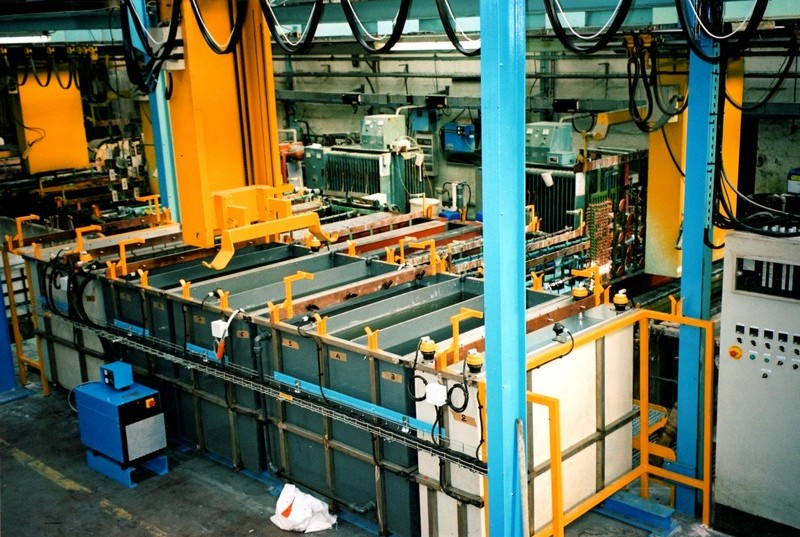
\includegraphics[width=0.7\linewidth]{img/Traitement1.jpg}
\end{minipage}
\hfill
\begin{minipage}{0.58\linewidth}
Un poste de dégraissage est utilisé pour décaper des pièces avant un traitement de surface. Ce poste se compose d'une zone de chargement, d'une zone de déchargement, d'une cuve de dégraissage et d'un chariot automoteur se déplaçant sur un rail. Ce chariot permet de déplacer un panier contenant les pièces à traiter. 

Le chargement et le déchargement du panier s'effectuent manuellement en position basse.
\end{minipage}

\begin{minipage}{0.5\linewidth}
La consigne de départ de cycle et l'information de fin de déchargement sont données manuellement par l'opérateur. 

Le chariot ne peut se déplacer que lorsque le panier est en position haute. Un voyant doit s'allumer lorsque le chariot se déplace. 

Les pièces doivent rester 30 secondes dans le bain de dégraissage. 

Le cycle ne peut démarrer que si le chariot est à gauche et le panier en bas.
\end{minipage}
\hfill
\begin{minipage}{0.48\linewidth}
 \centering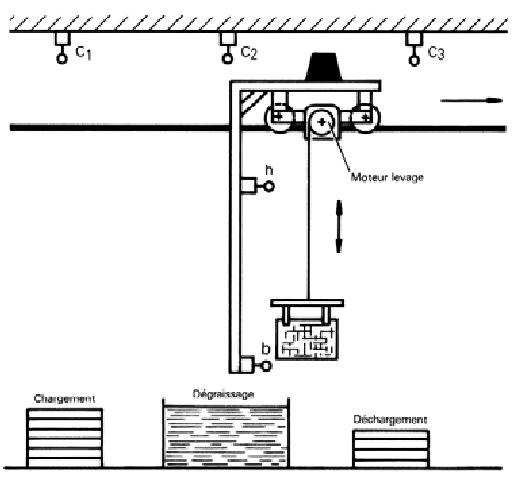
\includegraphics[width=0.7\linewidth]{img/Traitement2.png} 
\end{minipage}

\begin{tabular}{|c|c|c|c|}
\hline
\textbf{Consigne} & \textbf{Bouton poussoir} & \textbf{Signalisation} & \textbf{Voyant} \\
\hline
Départ de cycle donné & dcy & Allumer voyant & V \\
\hline
Panier déchargé & padech & & \\
\hline
\textbf{Compte rendu} & \textbf{Capteur} & \textbf{Ordre} & \textbf{Préactionneur} \\
\hline
Panier en haut & h & Avancer chariot & KM1 \\
\hline
Panier en bas & b & Reculer chariot & KM2 \\
\hline
Chariot en c1 & c1 & Monter panier & KM3 \\ 
\hline
Chariot en c2 & c2 & Descendre panier & KM4 \\
\hline
Chariot en c3 & c3 & & \\
\hline
\end{tabular}

\paragraph{Question 1:} Établir le diagramme d'activité du système:
\begin{itemize}
 \item Si l'opérateur donne comme consigne \og départ de cycle sans trempage \textbf{dcyst} \fg (au lieu de \og départ de cycle \textbf{dcy} \og), les pièces doivent être envoyées directement au poste de déchargement sans passer par le poste de dégraissage. 
\end{itemize}

\newpage

\section{Transfert rotatif de mise en pot}


\begin{minipage}{0.35\linewidth}
 \centering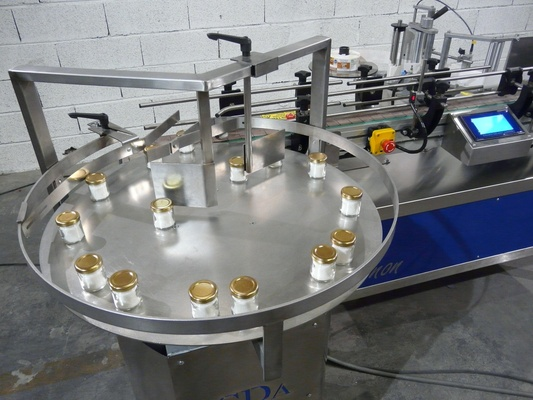
\includegraphics[width=0.9\linewidth]{img/Transfert1.jpg}
\end{minipage}
\hfill
\begin{minipage}{0.63\linewidth}
Les pots à remplir arrivent du poste de lavage sur le tapis d'amenage. 

Si le mode automatique est enclenché, les 3 tâches (Remplir, Boucher et Imprimer) sont effectuées simultanément. 

Ensuite dès que ces trois tâches sont terminées, les pots sont transférés d'un poste à l'autre (remplissage, bouchage, impression) par le disque de distribution motorisé par un motoréducteur.
\end{minipage}

~\

Une cellule photo-électrique détecte la position du disque. Ce dernier est en position lorsqu'un perçage est en face du détecteur. 

Un vérin indexeur pneumatique permet de maintenir en position le disque (voir zoom ci-dessous)). 

A l'étape initiale, on suppose que 3 pots sont déjà sous chaque poste. 

\begin{minipage}{0.48\linewidth}
 \centering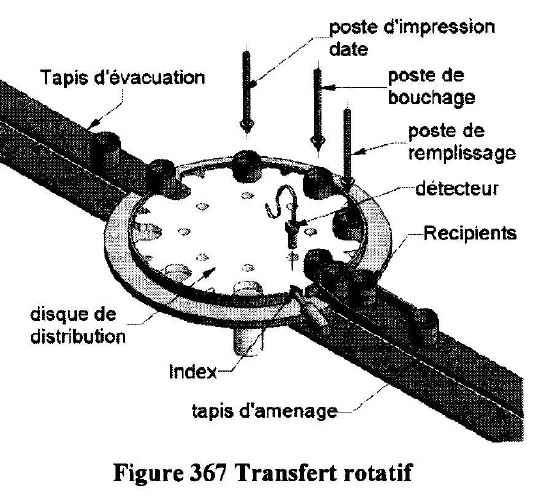
\includegraphics[width=0.7\linewidth]{img/Transfert2.png}
\end{minipage}
\hfill
\begin{minipage}{0.48\linewidth}
 \centering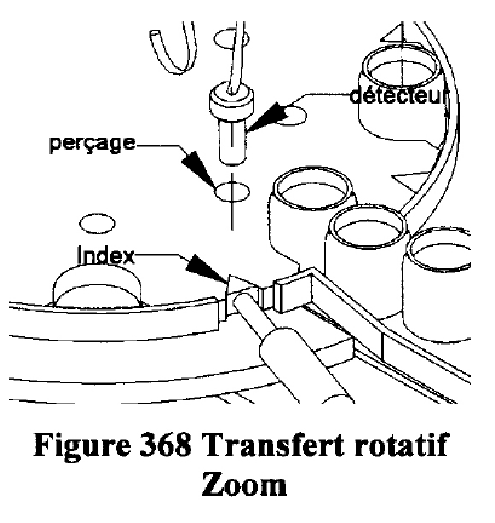
\includegraphics[width=0.7\linewidth]{img/Transfert3.png}
\end{minipage}


~\

\begin{center}
\begin{tabular}{|c|c|}
\hline
\textbf{Entrées} & \textbf{Sorties} \\
\hline
Fin remplissage & Remplir \\
\hline
Fin bouchage & Boucher \\
\hline
Fin impression & Imprimer \\
\hline
Disque désindexé & Désindexer \\
\hline
Disque indexé & Indexer \\
\hline
Position ok & Tourner disque \\
\hline
Automatique & \\
\hline
\end{tabular} 
\end{center}
 
\paragraph{Question 1:} A partir de la description du fonctionnement et de la carte des entrées sorties, déterminer le diagramme d'activité point de vue système utilisant les spécificités fonctionnelles de ce système. 
 

\clearpage

\ifdef{\public}{\end{document}}{}

\pagestyle{correction}

\newpage

\section{Correction}

\subsection{Palettiseur de gobelets}

\paragraph{Question 1:} Il faut $2^n-1>9999$ avec $n$ le plus petit possible. On trouve $n=14$. $2^{14}-1=16383$.

\paragraph{Question 2:}

\begin{center}
 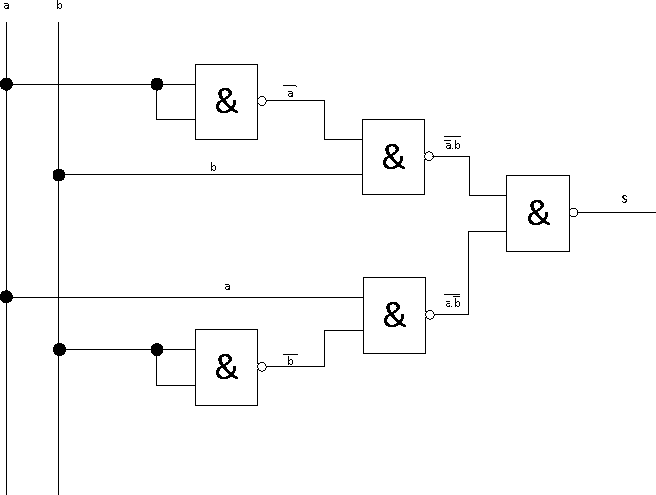
\includegraphics[width=0.7\linewidth]{img/nands}
\end{center}

\paragraph{Question 3:} $\overline{a \oplus b} = \overline{\overline{a}.b+a.\overline{b}}= \overline{\overline{a}.b}.\overline{a.\overline{b}} = (a+\overline{b}).(\overline{a}+b) = \overline{a}.\overline{b} + a.b$, car $\overline{a}.a=\overline{b}.b=0$.

\paragraph{Question 4:} $F(x,y,z,t,a,b,c,d)=\overline{x \oplus a}.\overline{y \oplus b}.\overline{z \oplus c}.\overline{t \oplus d}$

\paragraph{Question 5:}

\begin{itemize}
 \item $t2=vs1$
 \item $t5=vr2.vs3.\overline{cf}$
 \item $t'5=vr2.vs3.cf$
 \item $t7=vs1$
 \item $t10=vr2.vr3$
 \item $t11=ce$
\end{itemize}

\newpage

\paragraph{Question 6:}

\begin{center}
 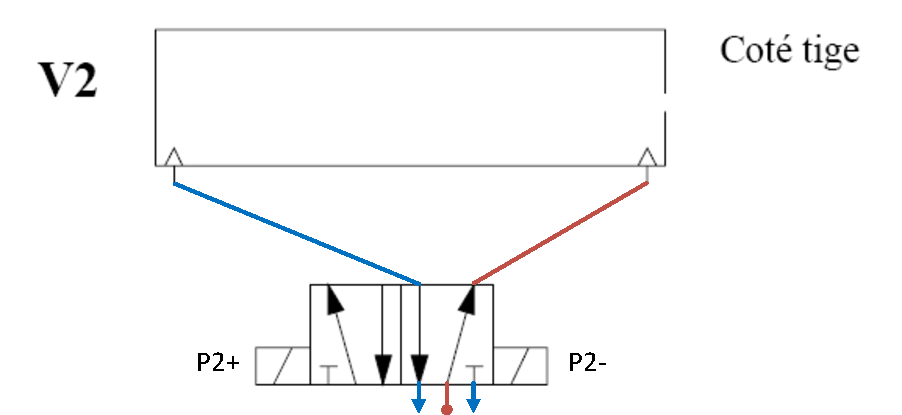
\includegraphics[width=0.7\linewidth]{img/distrib_cor}
\end{center}

\paragraph{Question 7:}

\begin{center}
 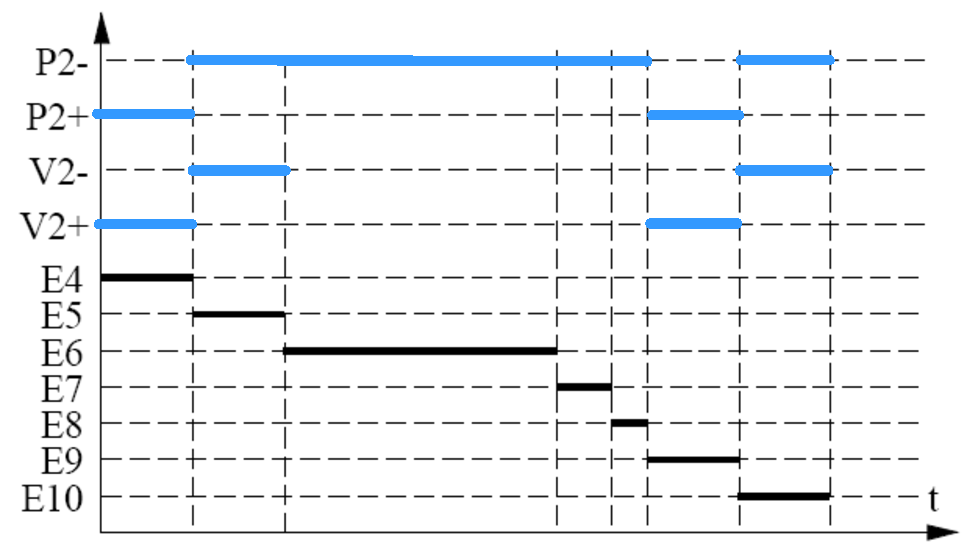
\includegraphics[width=0.7\linewidth]{img/chronogramme_cor}
\end{center}

\subsection{Robot robuglass}

\paragraph{Question 1:}

\begin{center}
 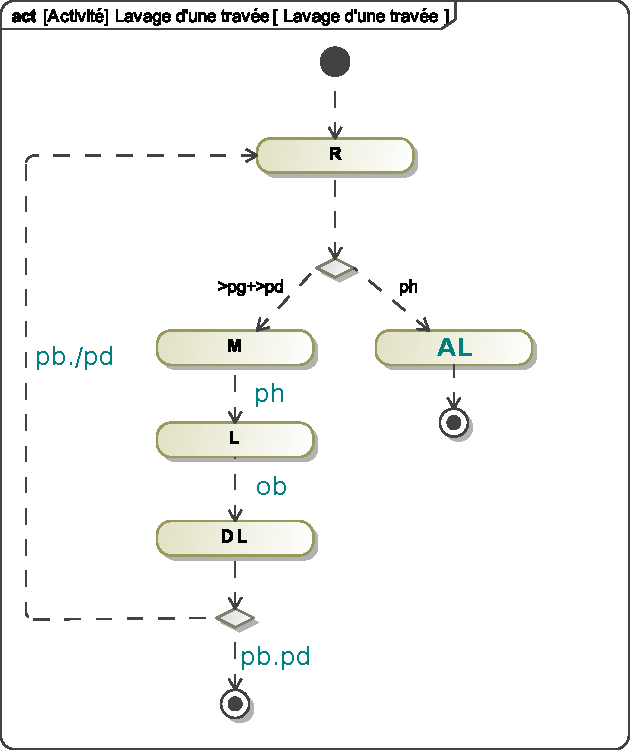
\includegraphics[width=0.7\linewidth]{img/Lavage_travee_cor}
\end{center}

\subsection{Traitement de surface}

\paragraph{Question 1:}

\begin{center}
 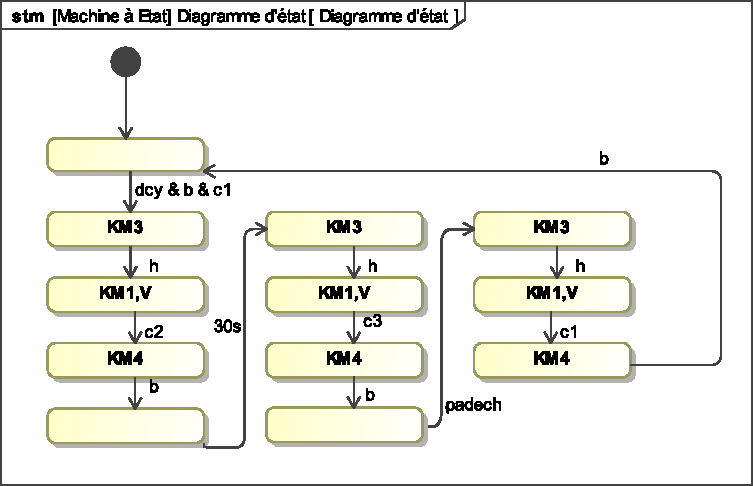
\includegraphics[width=0.7\linewidth]{img/traitement_cor}
\end{center}

\subsection{Transfert rotatif de mise en pot}

\paragraph{Question 1:}

\begin{center}
 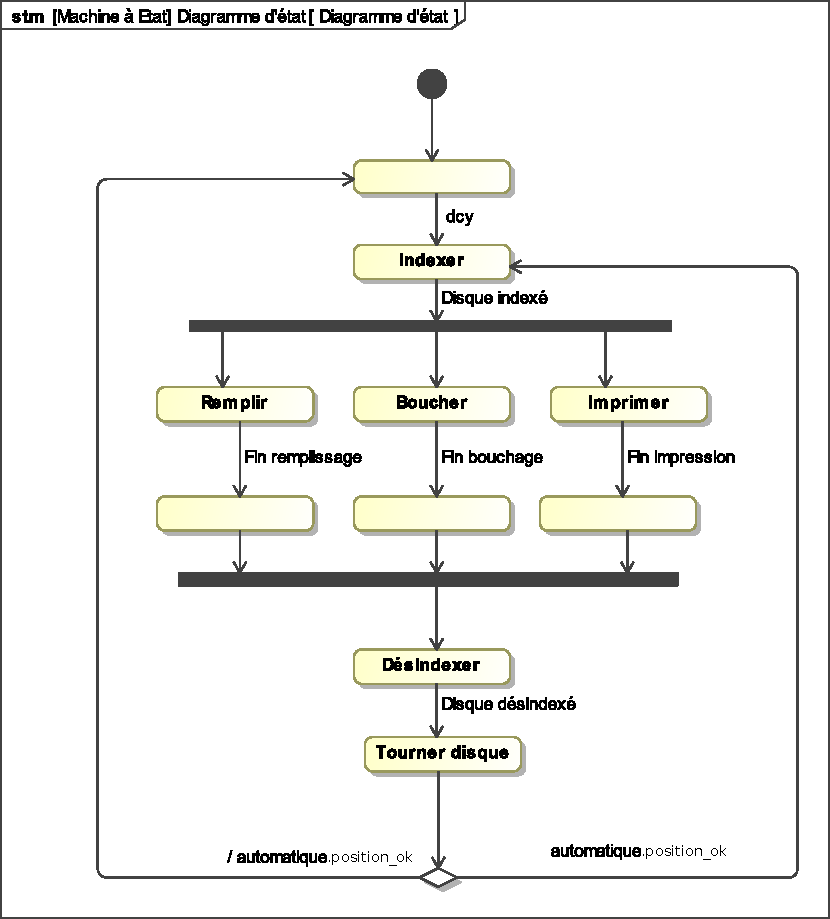
\includegraphics[width=0.7\linewidth]{img/remplir_pot_cor}
\end{center}

\end{document}
